\chapter{论文模板使用说明}
\graphicspath{{figures/chap02/}}
\section{论文模板简介}
本模板基于\LaTeX{}编写。 \LaTeX{}是一种基于\TeX{}的排版系统,由美国计算机科学家莱斯利·兰伯特在20世纪80年代初期开发 \cite{维基百科2020},它具有以下\CJKunderdot{优点}\cite{CTEX开发小组2020}:

\begin{itemize}
    \item 具有专业的排版输出能力,产生的文档看上去就像“印刷品”一样;
    \item 具有方便而强大的数学公式排版能力,无出其右者;
    \item 绝大多数时候,用户只需专注于一些组织文档结构的基础命令,无需(或很少)操心文档的版面设计;
    \item 很容易生成复杂的专业排版元素,如脚注、交叉引用、参考文献、目录等;
    \item 强大的可扩展性。世界各地的人开发了数以千计的 \LaTeX{} 宏包用于补充和扩展 \LaTeX{} 的功能;
    \item 能够促使用户写出结构良好的文档——而这也是 \LaTeX{} 存在的初衷;
    \item \LaTeX{} 和 \TeX{} 及相关软件是跨平台、免费、开源的;
    无论用户使用的是 Windows,macOS(OS X),GNU/Linux 还是 FreeBSD 等操作系统,都能轻松获得和使用这一强大的排版工具,并且获得稳定的输出。
  \end{itemize}

相较于Word排版系统,\LaTeX{}排版的优点显而易见。当然它也有一些缺点,比如不能所见即所得,入门门槛较高等,但笔者认为在进行长文档或是论文文档进行排版时,\LaTeX{}的效率是\texttt{Word}无法比拟的。事实上,国外相当多的期刊都接受\LaTeX{}投稿;国内也有部分期刊支持,但总的来说数量较少。此外,国内相当多的高校有着官方或非官方的学位论文模板,极大地便利了学生的论文写作。笔者相信本校学子也有或多或少的了解并有一定程度的使用,但时至今日\footnote{2020年夏}未见本校的学位论文模板,难免有些遗憾。在此情况下,笔者决定依据学校研究生学位论文写作要求撰写\LaTeX{}模板。

\section{使用建议}
\LaTeX{}的宏包非常多,可拓展出非常强大的制作和排版能力,例如\texttt{TikZ}等。关于\LaTeX{}具体使用本文档不作详细介绍,入门的同学推荐参考《一份(不太)简短的~\LaTeXe{}~介绍》\cite{CTEX开发小组2020},或是刘海洋编著的《\LaTeX{}入门》\cite{刘海洋2013}。欲作详细了解的可以查看《\LaTeX{}: A Document Preparation System or The \LaTeX{}~Companion》\cite{Lamport1994}和《The \LaTeX{}~Companion》\cite{Mittelbach2004}。关于宏包中的命令或特定功能的实现请阅读相应的宏包说明。
\section{问题与改进}
笔者所在专业为工程领域,对学校其它专业写作要求了解不多。另外本人也是\LaTeX{}排版系统入门者,撰写过程中也是边翻资料边学习命令,因此难免存在一些\textbf{\songti 错误和疏漏}。有兴趣使用的同学若在使用过程中出现问题,欢迎向笔者反映\footnote{个人邮箱:\texttt{chuandongxie@163.com},或\texttt{XAUATthesis}的\texttt{Github}代码仓};或是提出建议,笔者将不胜感激。

\section{工作示例}


\authornumcite{Berman2003}总结了多层钢板剪力墙的可能破坏模式,如图~\ref{fig:Berman2003}所示。其中,图~\ref{fig:Berman2003}(a)为薄弱层破坏模式:仅薄弱层处内填钢板屈服,层内柱端形成塑性铰,地震作用基本由薄弱层承担;图~\ref{fig:Berman2003}(b)为延性破坏模式:所有内填钢板均屈服,随后梁端形成塑性铰,最后柱脚形成塑性铰。同时,\authornumcite{Berman2003}提出了上述两种破坏模式的抗侧承载力计算方法。为避免钢板剪力墙结构体系发生薄弱层破坏,\authornumcite{Tsai2014}和\authornumcite{Li2014}提出采用端部削弱型的边框梁,并开展了理论分析与试验研究。然而,这些破坏模式中边框梁和边框柱都发生破坏,因此,震后该结构的可恢复性需进一步评估。

\begin{figure}[H] 
  \centering
  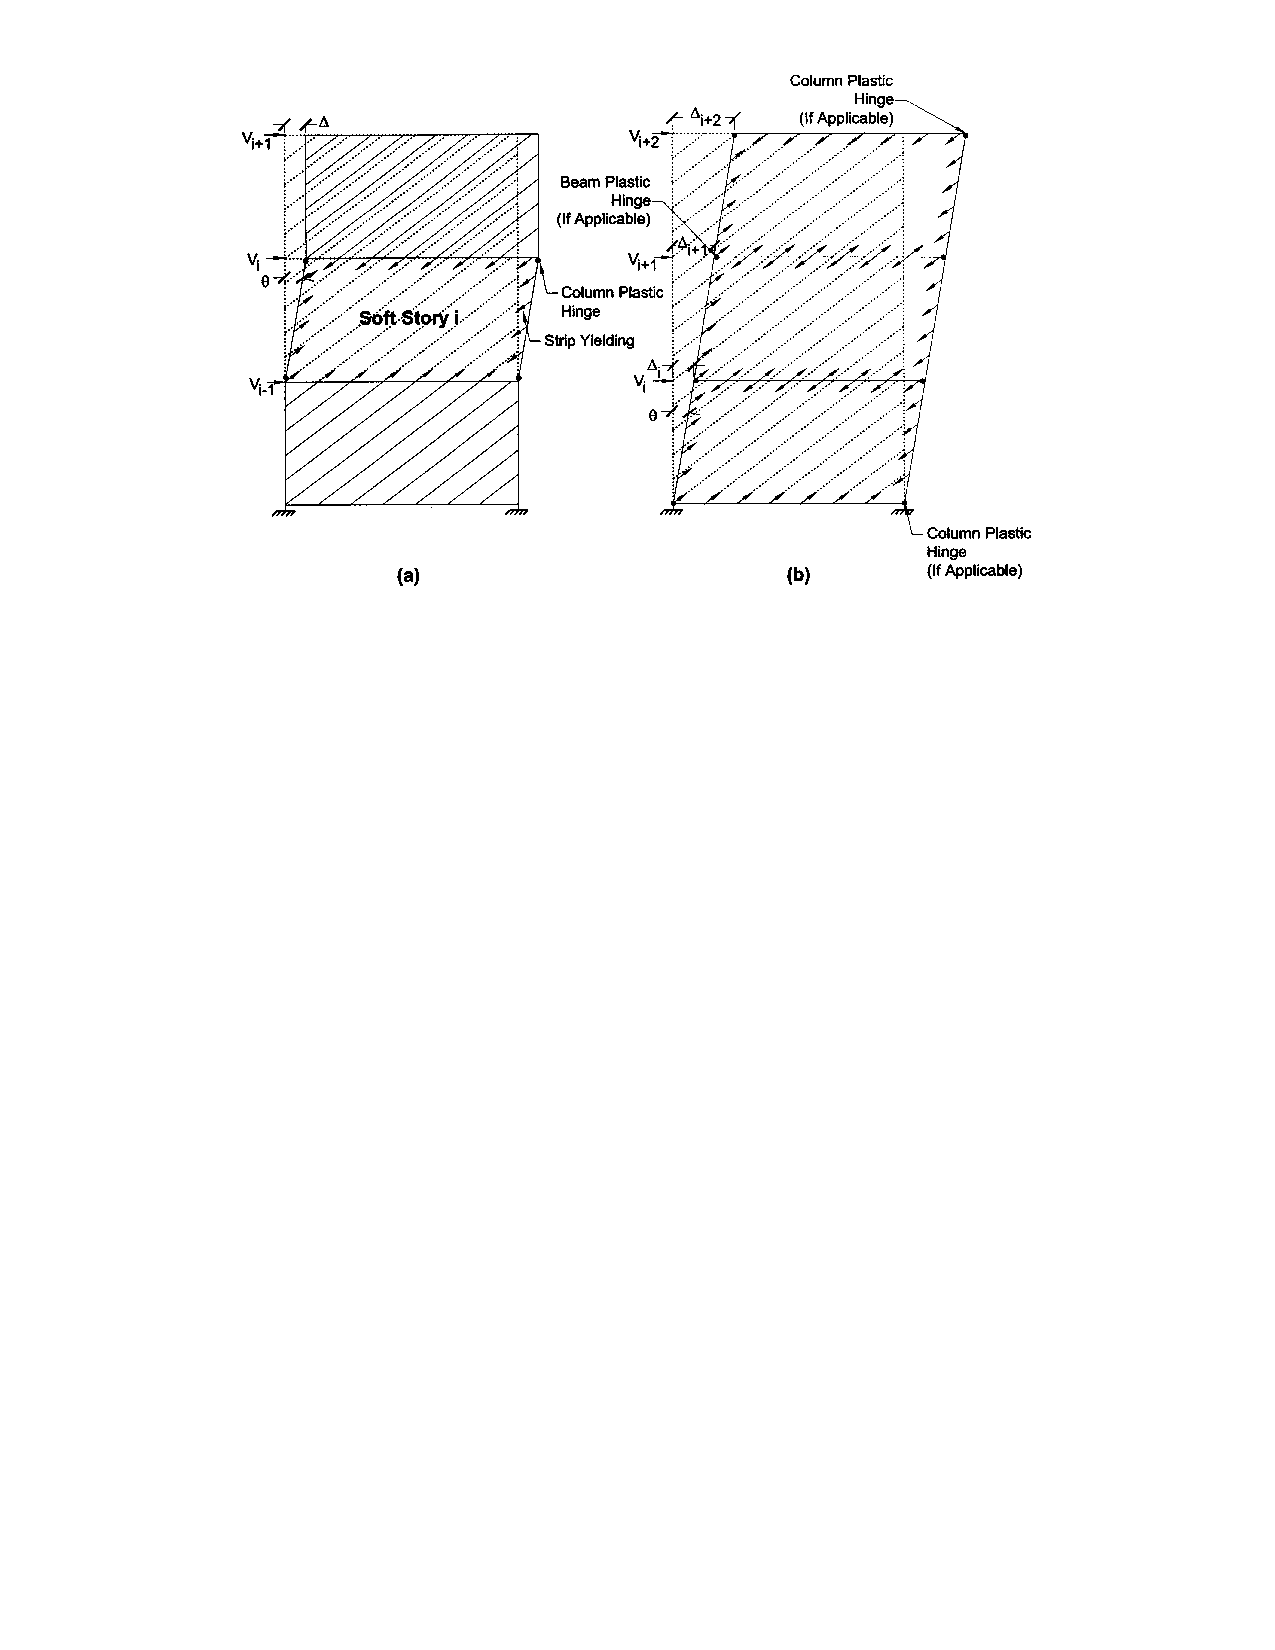
\includegraphics[width=12cm]{Berman2003.pdf}
  \bicaption{多层钢板剪力墙破坏模式}{Collapse mechanisms for multistory steel plate shear walls}
  \label{fig:Berman2003}
\end{figure}

在确定钢板剪力墙结构力学性能与设计方法时,较为关键的因素是拉力带倾角。\authornumcite{Thorburn1983}基于最小势能原理,提出了钢板剪力墙拉力带倾角计算公式:

\begin{equation}
\tan^4\alpha=\frac{1+\frac{Lw}{2A_{\rm{c}}}}{1+\frac{hw}{A_{\rm{b}}}}\qquad\mbox{(刚性边框柱)}
\label{Equ:1}
\end{equation}

\begin{equation}
\tan2\alpha=\frac{L}{H}\qquad\mbox{(柔性边框柱)}
\label{Equ:2}
\end{equation}

\authornumcite{Timler1983}考虑了边框柱有限刚度,对式~\ref{Equ:1}进行了修正:

\begin{equation}
\tan^4\alpha=\frac{1+\frac{Lw}{2A_{\rm{c}}}}{1+\left(\frac{1}{A_{\rm{b}}}+\frac{h^3}{360L_{\rm{c}}}\right)}
\label{Equ:3}
\end{equation}